\chapter{Test Cases and Results}
\label{sec:results}

Given the limitations outlined in section \ref{ssec:sol}, presently the ability
to do any kind of serious systems analysis with ADER is almost non-existent due
to the numerical stability issues inherent to the solution algorithm. Despite
this some configurations of system parameters may be found such that a simple
and limited simulation can be run to a sufficiently long time horizon to see
equilibrium within the fuel cycle.

\subsection{Simulation Setup}\label{ssec:setup}
The system configuration is described in this section with corresponding 
SERPENT 2
input provided in section \ref{ssec:input}. In short the simulation consisted
of an infinite and homogeneous salt mixture, 71.8 mol-\% \ce{LiF}, 16 mol-\%
\ce{BeF2}, 10.8 mol-\% \ce{ThF4}, and 1.2 mol-\% \ce{^{233}UF4} - the startup
fuel for the Oak Ridge Molten Salt Reactor Experiment \cite{ORNL}. The starting
lithium load was enriched to 99.995 \% \ce{^{7}Li}. The lithium
fraction of the homogeneous mixture was constrained to be between 0.26 and 0.30
using a range restriction. The total amount of lithium within the system was
tracked using a catch-all elemental group and a total summation group counting
both the lithium acting as a primary salt constituent and the lithium which may
be free or bound to fission products within the system. Separate groups of
elemental fluorine are used in ratio restrictions to impose chemical binding 
constraints on the Li, Be, Th, and U within the salt mixture. A free elemental
group of fluorine as well as a total fluorine summation group are used to track
total system fluorine. An elemental beryllium group constrains beryllium to
between 6.1 mol-\% and 6.5 mol-\%. The molar fractions of \ce{ThF4} as well
as \ce{UF4} - all uranium is assumed to be uranium-IV - are left free to vary
as ADER chooses. An oxidation range of $[-0.0002, -0.0001]$ is used to ensure
a reductive environment within the salt with each element's assumed oxidation
sate within the salt visually depicted in Figure \ref{periodic}. 
A mass balance is applied to the
system such that inflows must be equal, in number of mols, to outflows. Any
lithium, beryllium, fluorine, thorium-232, and uranium are required to be
represented in a group structure during the linear optimization. The
optimization target is set as the minimization of total gross flows.

The stream modelling natural removal removes the following elements into an 
infinite sink with a 30 second effective-half-life: He, Ne, Ar, Kr, Nb,
Mo, Tc, Ru, Rh, Pd, Ag, Sb, Te, Xe, and Rn. Those elements in the gas phase
given MSR operating temperatures and pressures - around one atmosphere and
generally between 550 $^{\circ}$ C and 800 $^{\circ}$ C - do not remain in
the salt and generally bubble out either in a Helium gas bubble trap or in the
pump bowl. The remaining elements in the natural removal stream are considered
the `noble' metals and will plate out, most commonly, on the cold leg of a flow
loop. Previous modelling by \cite{Aufiero} has shown that the 30 second
effective half-life captures these physical effects well. Figure 
\ref{fig:periodic} provides a visual depiction of the natural removal stream,
the reprocessing stream, as well as the assumed oxidation state of each element
in the salt which is seen in the upper right corner of each element's box and
for which a number not preceded by a minus sign indicates an oxidized state.
All elements, other than the chalcogens and halogens, are assumed to be in 
their highest oxidation state unless operational data from \cite{ORNL} 
indicates otherwise.

The stream modelling the reprocessing of the fuel salt removes the following
elements into an infinite sink: B, N, C, O, Na, Mg, Al, Si, P, S, Cl, K, Ca, Sc,
Ti, V, Cr, Mn, Fe, Co, Ni, Cu, Lu, Hf, Ta, W, Re, Os, Ir, Pt, Au, Hg, Tl, Pb,
Bi, Po, At, Fr, Ra, Lr, Rf, Db, Sg, Bh, Hs, Mt, Ac, Pa, Zn, Ga, Ge, As, Se, Br,
Rb, Sr, Y, Zr, Cd, In, Sn, I, La, Ce, Pr, Nd, Pm, Sm, Eu, Gd, Tb, Dy, Ho, Er,
Tm, Yb, Cs, and Ba. This removal occurs such that half of each element's total
abundance is removed every 10 years. 

The remaining streams in this simulation are all group-class streams whose
quantity is determined on a per burnup step basis by the linear optimization
routine. All of these remaining streams inject or remove their assigned quantity
of material at a continuous and unchanged rate with respect to time. These
remaining streams are a lithium injection stream enriched to 99.995 \% 
\ce{^{7}Li}, an elemental \ce{LiF} removal stream, a \ce{^{9}Be} injection
stream, an elemental \ce{BeF2} removal stream, a \ce{^{19}F} injection stream, 
an elemental fluorine removal stream, a \ce{^{232}ThF4} injection stream, an
elemental \ce{ThF4} removal stream, a \ce{^{233}UF4} injection stream, and an
elemental \ce{UF4} removal stream.

With regards to simulation parameters, the burnup steps were measured in days
and grew in length according to the Fibonacci sequence up to 34 days at which
each remaining burnup step was kept to 34 days. The minimum and maximum 
neutron multiplication factor targets were 1.0 and 1.01 respectively. A linear
extrapolation and interpolation scheme was selected for the nuclear cross
sections used in the standard CRAM burnup calculation. All possible nuclides
were tracked. Each monte-carlo system simulation was run with 10k neutrons for
40 inactive cycles with 60 active cycles; average cycle error on neutron
multiplication was approximately 150 pcm. Simulations were carried out on the
Savior HPC cluster here at UC Berkeley on a Dell PowerEdge C6220 server blade
equipped with two Intel Xenon 10-core Ivy Bridge processors all running at
2.5 GHz having 64 GB of memory.

\begin{figure} \label{fig:periodic}
\begin{centering}
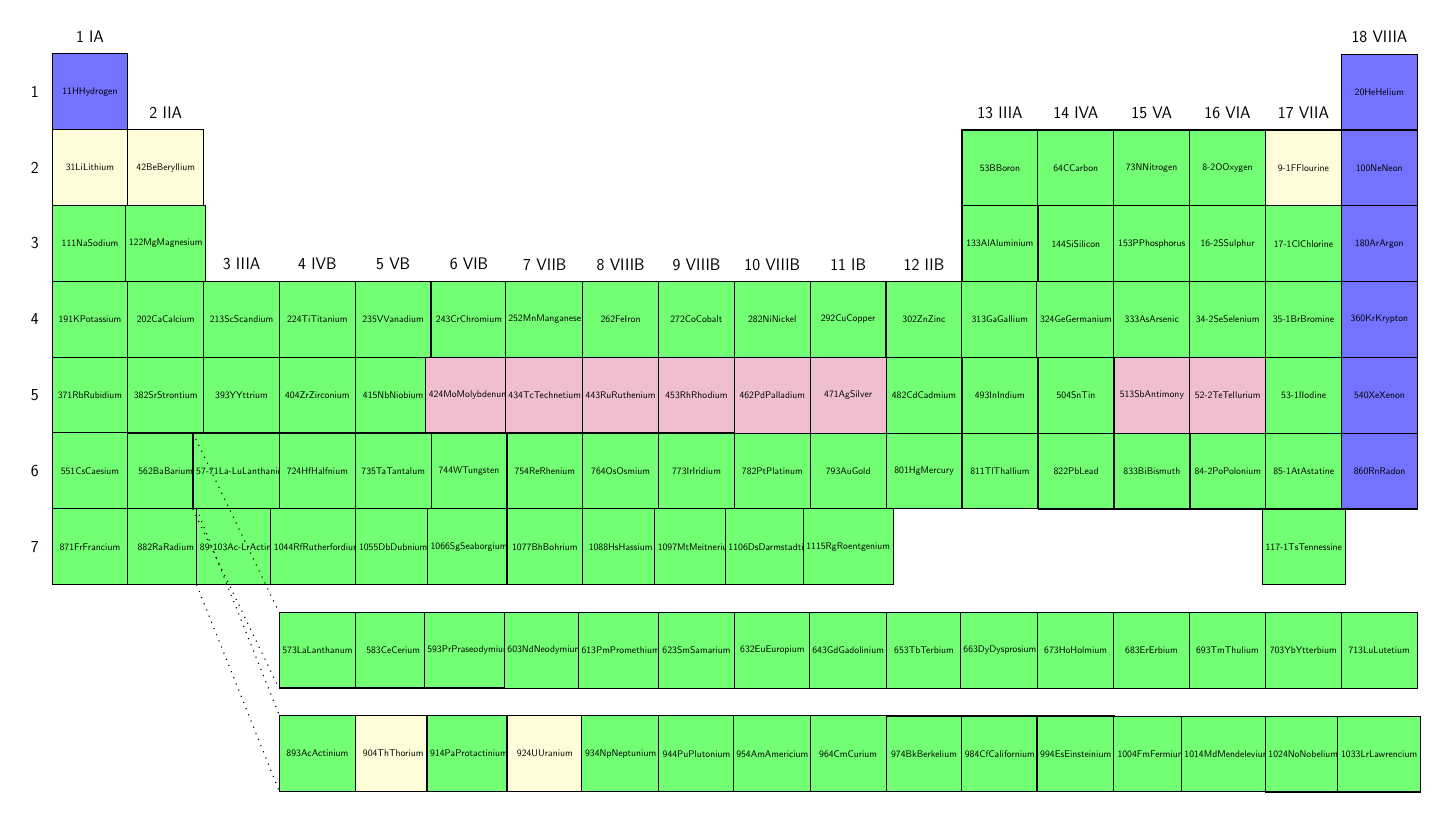
\begin{tikzpicture}[font=\sffamily, scale=0.35, transform shape]

%% Fill Color Styles
  \tikzstyle{ElementFill} = [fill=yellow!15]
  \tikzstyle{AlkaliMetalFill} = [fill=green!55]
  \tikzstyle{AlkalineEarthMetalFill} = [fill=green!55]
  \tikzstyle{MetalFill} = [fill=green!55]
  \tikzstyle{MetalloidFill} = [fill=green!55]
  \tikzstyle{NonmetalFill} = [fill=green!55]
  \tikzstyle{HalogenFill} = [fill=green!55]
  \tikzstyle{NobleGasFill} = [fill=green!55]
  \tikzstyle{LanthanideActinideFill} = [fill=green!55]
  \tikzstyle{B} = [fill=blue!55]
  \tikzstyle{N} = [fill=purple!25]
  \tikzstyle{F} = [fill=green!55]

%% Element Styles
  \tikzstyle{Element} = [draw=black, ElementFill,
    minimum width=2.75cm, minimum height=2.75cm, node distance=2.75cm]
  \tikzstyle{AlkaliMetal} = [Element, AlkaliMetalFill]
  \tikzstyle{AlkalineEarthMetal} = [Element, AlkalineEarthMetalFill]
  \tikzstyle{Metal} = [Element, MetalFill]
  \tikzstyle{Metalloid} = [Element, MetalloidFill]
  \tikzstyle{Nonmetal} = [Element, NonmetalFill]
  \tikzstyle{Halogen} = [Element, HalogenFill]
  \tikzstyle{NobleGas} = [Element, NobleGasFill]
  \tikzstyle{LanthanideActinide} = [Element, LanthanideActinideFill]
  \tikzstyle{PeriodLabel} = [font={\sffamily\LARGE}, node distance=2.0cm]
  \tikzstyle{GroupLabel} = [font={\sffamily\LARGE}, minimum width=2.75cm, node distance=2.0cm]
  \tikzstyle{TitleLabel} = [font={\sffamily\Huge\bfseries}]
  \tikzstyle{b} = [Element, B]
  \tikzstyle{n} = [Element, N]
  \tikzstyle{f} = [Element, F]

%% Group 1 - IA
  \node[name=H, b] {\NaturalElementTextFormat{1}{1}{H}{Hydrogen}};
  \node[name=Li, below of=H, Element] {\NaturalElementTextFormat{3}{1}{Li}{Lithium}};
  \node[name=Na, below of=Li, AlkaliMetal] {\NaturalElementTextFormat{11}{1}{Na}{Sodium}};
  \node[name=K, below of=Na, AlkaliMetal] {\NaturalElementTextFormat{19}{1}{K}{Potassium}};
  \node[name=Rb, below of=K, AlkaliMetal] {\NaturalElementTextFormat{37}{1}{Rb}{Rubidium}};
  \node[name=Cs, below of=Rb, AlkaliMetal] {\NaturalElementTextFormat{55}{1}{Cs}{Caesium}};
  \node[name=Fr, below of=Cs, AlkaliMetal] {\NaturalElementTextFormat{87}{1}{Fr}{Francium}};

%% Group 2 - IIA
  \node[name=Be, right of=Li, Element] {\NaturalElementTextFormat{4}{2}{Be}{Beryllium}};
  \node[name=Mg, below of=Be, AlkalineEarthMetal] {\NaturalElementTextFormat{12}{2}{Mg}{Magnesium}};
  \node[name=Ca, below of=Mg, AlkalineEarthMetal] {\NaturalElementTextFormat{20}{2}{Ca}{Calcium}};
  \node[name=Sr, below of=Ca, AlkalineEarthMetal] {\NaturalElementTextFormat{38}{2}{Sr}{Strontium}};
  \node[name=Ba, below of=Sr, AlkalineEarthMetal] {\NaturalElementTextFormat{56}{2}{Ba}{Barium}};
  \node[name=Ra, below of=Ba, AlkalineEarthMetal] {\NaturalElementTextFormat{88}{2}{Ra}{Radium}};

%% Group 3 - IIIB
  \node[name=Sc, right of=Ca, Metal] {\NaturalElementTextFormat{21}{3}{Sc}{Scandium}};
  \node[name=Y, below of=Sc, Metal] {\NaturalElementTextFormat{39}{3}{Y}{Yttrium}};
  \node[name=LaLu, below of=Y, LanthanideActinide] {\NaturalElementTextFormat{57-71}{}{La-Lu}{Lanthanide}};
  \node[name=AcLr, below of=LaLu, LanthanideActinide] {\NaturalElementTextFormat{89-103}{}{Ac-Lr}{Actinide}};

%% Group 4 - IVB
  \node[name=Ti, right of=Sc, Metal] {\NaturalElementTextFormat{22}{4}{Ti}{Titanium}};
  \node[name=Zr, below of=Ti, Metal] {\NaturalElementTextFormat{40}{4}{Zr}{Zirconium}};
  \node[name=Hf, below of=Zr, Metal] {\NaturalElementTextFormat{72}{4}{Hf}{Halfnium}};
  \node[name=Rf, below of=Hf, Metal] {\SyntheticElementTextFormat{104}{4}{Rf}{Rutherfordium}};

%% Group 5 - VB
  \node[name=V, right of=Ti, Metal] {\NaturalElementTextFormat{23}{5}{V}{Vanadium}};
  \node[name=Nb, below of=V, Metal] {\NaturalElementTextFormat{41}{5}{Nb}{Niobium}};
  \node[name=Ta, below of=Nb, Metal] {\NaturalElementTextFormat{73}{5}{Ta}{Tantalum}};
  \node[name=Db, below of=Ta, Metal] {\SyntheticElementTextFormat{105}{5}{Db}{Dubnium}};

%% Group 6 - VIB
  \node[name=Cr, right of=V, Metal] {\NaturalElementTextFormat{24}{3}{Cr}{Chromium}};
  \node[name=Mo, below of=Cr, n] {\NaturalElementTextFormat{42}{4}{Mo}{Molybdenum}};
  \node[name=W, below of=Mo, Metal] {\NaturalElementTextFormat{74}{4}{W}{Tungsten}};
  \node[name=Sg, below of=W, Metal] {\SyntheticElementTextFormat{106}{6}{Sg}{Seaborgium}};

%% Group 7 - VIIB
  \node[name=Mn, right of=Cr, Metal] {\NaturalElementTextFormat{25}{2}{Mn}{Manganese}};
  \node[name=Tc, below of=Mn, n] {\NaturalElementTextFormat{43}{4}{Tc}{Technetium}};
  \node[name=Re, below of=Tc, Metal] {\NaturalElementTextFormat{75}{4}{Re}{Rhenium}};
  \node[name=Bh, below of=Re, Metal] {\SyntheticElementTextFormat{107}{7}{Bh}{Bohrium}};

%% Group 8 - VIIIB
  \node[name=Fe, right of=Mn, Metal] {\NaturalElementTextFormat{26}{2}{Fe}{Iron}};
  \node[name=Ru, below of=Fe, n] {\NaturalElementTextFormat{44}{3}{Ru}{Ruthenium}};
  \node[name=Os, below of=Ru, Metal] {\NaturalElementTextFormat{76}{4}{Os}{Osmium}};
  \node[name=Hs, below of=Os, Metal] {\SyntheticElementTextFormat{108}{8}{Hs}{Hassium}};

%% Group 9 - VIIIB
  \node[name=Co, right of=Fe, Metal] {\NaturalElementTextFormat{27}{2}{Co}{Cobalt}};
  \node[name=Rh, below of=Co, n] {\NaturalElementTextFormat{45}{3}{Rh}{Rhodium}};
  \node[name=Ir, below of=Rh, Metal] {\NaturalElementTextFormat{77}{3}{Ir}{Iridium}};
  \node[name=Mt, below of=Ir, Metal] {\SyntheticElementTextFormat{109}{7}{Mt}{Meitnerium}};

%% Group 10 - VIIIB
  \node[name=Ni, right of=Co, Metal] {\NaturalElementTextFormat{28}{2}{Ni}{Nickel}};
  \node[name=Pd, below of=Ni, n] {\NaturalElementTextFormat{46}{2}{Pd}{Palladium}};
  \node[name=Pt, below of=Pd, Metal] {\NaturalElementTextFormat{78}{2}{Pt}{Platinum}};
  \node[name=Ds, below of=Pt, Metal] {\SyntheticElementTextFormat{110}{6}{Ds}{Darmstadtium}};

%% Group 11 - IB
  \node[name=Cu, right of=Ni, Metal] {\NaturalElementTextFormat{29}{2}{Cu}{Copper}};
  \node[name=Ag, below of=Cu, n] {\NaturalElementTextFormat{47}{1}{Ag}{Silver}};
  \node[name=Au, below of=Ag, Metal] {\NaturalElementTextFormat{79}{3}{Au}{Gold}};
  \node[name=Rg, below of=Au, Metal] {\SyntheticElementTextFormat{111}{5}{Rg}{Roentgenium}};

%% Group 12 - IIB
  \node[name=Zn, right of=Cu, Metal] {\NaturalElementTextFormat{30}{2}{Zn}{Zinc}};
  \node[name=Cd, below of=Zn, Metal] {\NaturalElementTextFormat{48}{2}{Cd}{Cadmium}};
  \node[name=Hg, below of=Cd, Metal] {\NaturalElementTextFormat{80}{1}{Hg}{Mercury}};

%% Group 13 - IIIA
  \node[name=Ga, right of=Zn, Metal] {\NaturalElementTextFormat{31}{3}{Ga}{Gallium}};
  \node[name=Al, above of=Ga, Metal] {\NaturalElementTextFormat{13}{3}{Al}{Aluminium}};
  \node[name=B, above of=Al, Metalloid] {\NaturalElementTextFormat{5}{3}{B}{Boron}};
  \node[name=In, below of=Ga, Metal] {\NaturalElementTextFormat{49}{3}{In}{Indium}};
  \node[name=Tl, below of=In, Metal] {\NaturalElementTextFormat{81}{1}{Tl}{Thallium}};

%% Group 14 - IVA
  \node[name=C, right of=B, Nonmetal] {\NaturalElementTextFormat{6}{4}{C}{Carbon}};
  \node[name=Si, below of=C, Metalloid] {\NaturalElementTextFormat{14}{4}{Si}{Silicon}};
  \node[name=Ge, below of=Si, Metalloid] {\NaturalElementTextFormat{32}{4}{Ge}{Germanium}};
  \node[name=Sn, below of=Ge, Metal] {\NaturalElementTextFormat{50}{4}{Sn}{Tin}};
  \node[name=Pb, below of=Sn, Metal] {\NaturalElementTextFormat{82}{2}{Pb}{Lead}};

%% Group 15 - VA
  \node[name=N, right of=C, Nonmetal] {\NaturalElementTextFormat{7}{3}{N}{Nitrogen}};
  \node[name=P, below of=N, Nonmetal] {\NaturalElementTextFormat{15}{3}{P}{Phosphorus}};
  \node[name=As, below of=P, Metalloid] {\NaturalElementTextFormat{33}{3}{As}{Arsenic}};
  \node[name=Sb, below of=As, n] {\NaturalElementTextFormat{51}{3}{Sb}{Antimony}};
  \node[name=Bi, below of=Sb, Metal] {\NaturalElementTextFormat{83}{3}{Bi}{Bismuth}};

%% Group 16 - VIA
  \node[name=O, right of=N, Nonmetal] {\NaturalElementTextFormat{8}{-2}{O}{Oxygen}};
  \node[name=S, below of=O, Nonmetal] {\NaturalElementTextFormat{16}{-2}{S}{Sulphur}};
  \node[name=Se, below of=S, Nonmetal] {\NaturalElementTextFormat{34}{-2}{Se}{Selenium}};
  \node[name=Te, below of=Se, n] {\NaturalElementTextFormat{52}{-2}{Te}{Tellurium}};
  \node[name=Po, below of=Te, Metalloid] {\NaturalElementTextFormat{84}{-2}{Po}{Polonium}};

%% Group 17 - VIIA
  \node[name=F, right of=O, Element] {\NaturalElementTextFormat{9}{-1}{F}{Flourine}};
  \node[name=Cl, below of=F, Halogen] {\NaturalElementTextFormat{17}{-1}{Cl}{Chlorine}};
  \node[name=Br, below of=Cl, Halogen] {\NaturalElementTextFormat{35}{-1}{Br}{Bromine}};
  \node[name=I, below of=Br, Halogen] {\NaturalElementTextFormat{53}{-1}{I}{Iodine}};
  \node[name=At, below of=I, Halogen] {\NaturalElementTextFormat{85}{-1}{At}{Astatine}};
  \node[name=Ts, below of=At, Halogen] {\SyntheticElementTextFormat{117}{-1}{Ts}{Tennessine}}; 

%% Group 18 - VIIIA
  \node[name=Ne, right of=F, b] {\NaturalElementTextFormat{10}{0}{Ne}{Neon}};
  \node[name=He, above of=Ne, b] {\NaturalElementTextFormat{2}{0}{He}{Helium}};
  \node[name=Ar, below of=Ne, b] {\NaturalElementTextFormat{18}{0}{Ar}{Argon}};
  \node[name=Kr, below of=Ar, b] {\NaturalElementTextFormat{36}{0}{Kr}{Krypton}};
  \node[name=Xe, below of=Kr, b] {\NaturalElementTextFormat{54}{0}{Xe}{Xenon}};
  \node[name=Rn, below of=Xe, b] {\NaturalElementTextFormat{86}{0}{Rn}{Radon}};

%% Period
  \node[name=Period1, left of=H, PeriodLabel] {1};
  \node[name=Period2, left of=Li, PeriodLabel] {2};
  \node[name=Period3, left of=Na, PeriodLabel] {3}; 
  \node[name=Period4, left of=K, PeriodLabel] {4}; 
  \node[name=Period5, left of=Rb, PeriodLabel] {5};
  \node[name=Period6, left of=Cs, PeriodLabel] {6};
  \node[name=Period7, left of=Fr, PeriodLabel] {7};

%% Group
  \node[name=Group1, above of=H, GroupLabel] {1 \hfill IA};
  \node[name=Group2, above of=Be, GroupLabel] {2 \hfill IIA};
  \node[name=Group3, above of=Sc, GroupLabel] {3 \hfill IIIA};
  \node[name=Group4, above of=Ti, GroupLabel] {4 \hfill IVB};
  \node[name=Group5, above of=V, GroupLabel] {5 \hfill VB};
  \node[name=Group6, above of=Cr, GroupLabel] {6 \hfill VIB};
  \node[name=Group7, above of=Mn, GroupLabel] {7 \hfill VIIB};
  \node[name=Group8, above of=Fe, GroupLabel] {8 \hfill VIIIB};
  \node[name=Group9, above of=Co, GroupLabel] {9 \hfill VIIIB};
  \node[name=Group10, above of=Ni, GroupLabel] {10 \hfill VIIIB};
  \node[name=Group11, above of=Cu, GroupLabel] {11 \hfill IB};
  \node[name=Group12, above of=Zn, GroupLabel] {12 \hfill IIB};
  \node[name=Group13, above of=B, GroupLabel] {13 \hfill IIIA};
  \node[name=Group14, above of=C, GroupLabel] {14 \hfill IVA};
  \node[name=Group15, above of=N, GroupLabel] {15 \hfill VA};
  \node[name=Group16, above of=O, GroupLabel] {16 \hfill VIA};
  \node[name=Group17, above of=F, GroupLabel] {17 \hfill VIIA};
  \node[name=Group18, above of=He, GroupLabel] {18 \hfill VIIIA};

%% Lanthanide
  \node[name=La, below of=Rf, LanthanideActinide, yshift=-1cm] {\NaturalElementTextFormat{57}{3}{La}{Lanthanum}};
  \node[name=Ce, right of=La, LanthanideActinide] {\NaturalElementTextFormat{58}{3}{Ce}{Cerium}};
  \node[name=Pr, right of=Ce, LanthanideActinide] {\NaturalElementTextFormat{59}{3}{Pr}{Praseodymium}};
  \node[name=Nd, right of=Pr, LanthanideActinide] {\NaturalElementTextFormat{60}{3}{Nd}{Neodymium}};
  \node[name=Pm, right of=Nd, LanthanideActinide] {\NaturalElementTextFormat{61}{3}{Pm}{Promethium}};
  \node[name=Sm, right of=Pm, LanthanideActinide] {\NaturalElementTextFormat{62}{3}{Sm}{Samarium}};
  \node[name=Eu, right of=Sm, LanthanideActinide] {\NaturalElementTextFormat{63}{2}{Eu}{Europium}};
  \node[name=Gd, right of=Eu, LanthanideActinide] {\NaturalElementTextFormat{64}{3}{Gd}{Gadolinium}};
  \node[name=Tb, right of=Gd, LanthanideActinide] {\NaturalElementTextFormat{65}{3}{Tb}{Terbium}};
  \node[name=Dy, right of=Tb, LanthanideActinide] {\NaturalElementTextFormat{66}{3}{Dy}{Dysprosium}};
  \node[name=Ho, right of=Dy, LanthanideActinide] {\NaturalElementTextFormat{67}{3}{Ho}{Holmium}};
  \node[name=Er, right of=Ho, LanthanideActinide] {\NaturalElementTextFormat{68}{3}{Er}{Erbium}};
  \node[name=Tm, right of=Er, LanthanideActinide] {\NaturalElementTextFormat{69}{3}{Tm}{Thulium}};
  \node[name=Yb, right of=Tm, LanthanideActinide] {\NaturalElementTextFormat{70}{3}{Yb}{Ytterbium}};
  \node[name=Lu, right of=Yb, LanthanideActinide] {\NaturalElementTextFormat{71}{3}{Lu}{Lutetium}};

%% Actinide
  \node[name=Ac, below of=La, LanthanideActinide, yshift=-1cm] {\NaturalElementTextFormat{89}{3}{Ac}{Actinium}};
  \node[name=Th, right of=Ac, Element] {\NaturalElementTextFormat{90}{4}{Th}{Thorium}};
  \node[name=Pa, right of=Th, LanthanideActinide] {\NaturalElementTextFormat{91}{4}{Pa}{Protactinium}};
  \node[name=U, right of=Pa, Element] {\NaturalElementTextFormat{92}{4}{U}{Uranium}};
  \node[name=Np, right of=U, LanthanideActinide] {\SyntheticElementTextFormat{93}{4}{Np}{Neptunium}};
  \node[name=Pu, right of=Np, LanthanideActinide] {\SyntheticElementTextFormat{94}{4}{Pu}{Plutonium}};
  \node[name=Am, right of=Pu, LanthanideActinide] {\SyntheticElementTextFormat{95}{4}{Am}{Americium}};
  \node[name=Cm, right of=Am, LanthanideActinide] {\SyntheticElementTextFormat{96}{4}{Cm}{Curium}};
  \node[name=Bk, right of=Cm, LanthanideActinide] {\SyntheticElementTextFormat{97}{4}{Bk}{Berkelium}};
  \node[name=Cf, right of=Bk, LanthanideActinide] {\SyntheticElementTextFormat{98}{4}{Cf}{Californium}};
  \node[name=Es, right of=Cf, LanthanideActinide] {\SyntheticElementTextFormat{99}{4}{Es}{Einsteinium}};
  \node[name=Fm, right of=Es, LanthanideActinide] {\SyntheticElementTextFormat{100}{4}{Fm}{Fermium}};
  \node[name=Md, right of=Fm, LanthanideActinide] {\SyntheticElementTextFormat{101}{4}{Md}{Mendelevium}};
  \node[name=No, right of=Md, LanthanideActinide] {\SyntheticElementTextFormat{102}{4}{No}{Nobelium}};
  \node[name=Lr, right of=No, LanthanideActinide] {\SyntheticElementTextFormat{103}{3}{Lr}{Lawrencium}};

%% Draw dotted lines connecting Lanthanide breakout to main table
  \draw (LaLu.north west) edge[dotted] (La.north west)
   %     (LaLu.north east) edge[dotted] (Lu.north east)
        (LaLu.south west) edge[dotted] (La.south west);
   %     (LaLu.south east) edge[dotted] (Lu.south east);
%% Draw dotted lines connecting Actinide breakout to main table
  \draw (AcLr.north west) edge[dotted] (Ac.north west)
   %     (AcLr.north east) edge[dotted] (Lr.north east)
        (AcLr.south west) edge[dotted] (Ac.south west);
   %     (AcLr.south east) edge[dotted] (Lr.south east);

\end{tikzpicture}
\end{centering}
\caption{Elements in blue are those which bubble out of the salt and are
included in the natural processes removal stream as are elements in light-red
as these are the `noble' metals which are insoluble in the salt. Elements in
green are considered fission products of which 50\% are removed every ten
years. Periodic table layout in TikZ provided by Chris Rump and Ivan Griffin
through overleaf.com}
\end{figure}

\subsection{Simulation Outputs}\label{ssec:outputs}

In Figures \ref{fig:fuel} through \ref{fig:k} the results of the simulation
described in section \ref{ssec:setup} - with input given in Appendix
\ref{app:input} - are given below. Following this presentation in section
\ref{ssec:disc} the lessons learned from these figures and outputs are
given. The units given for group and stream values, $\%-\rho^{mat}_{i}$, are
relative fractions of the host material, $mat$, density as measured at the 
beginning of burnup step $i$.

\begin{figure}[H]
    \centering
    \includegraphics[width=0.8\textwidth]{fuel}
    \caption{The primary fuel constituents - Li (yellow), Be (purple), F (red),
    U (green), Th (blue) - atom density over the entire simulation.}
    \label{fig:fuel}
\end{figure}

\begin{figure}[H]
    \centering
    \includegraphics[width=0.8\textwidth]{fp}
    \caption{As described in section \ref{ssec:setup} and visually seen in
    Figure \ref{fig:periodic} here is seen the atomic density of all elements
    in the salt considered to be fission products.}
    \label{fig:fp}
\end{figure}

\begin{figure}[H]
    \centering
    \includegraphics[width=0.8\textwidth]{nat}
    \caption{The atomic density of the sum total of elements removed from the
    system by the stream used to simulate natural removal processes.}
    \label{fig:nat}
\end{figure}

\begin{figure}[H]
    \centering
    \includegraphics[width=0.8\textwidth]{proc}
    \caption{The atomic density of the sum total of elements removed from the
    system by the stream used to simulate a reprocessing function applied to
    the fuel salt.}
    \label{fig:proc}
\end{figure}

\begin{figure}[H]
    \centering
    \includegraphics[width=0.8\textwidth]{GgLiS}
    \caption{The atomic density of lithium elements considered to be a primary
    salt constituent.}
    \label{fig:GgLiS}
\end{figure}

\begin{figure}[H]
    \centering
    \includegraphics[width=0.8\textwidth]{GgLi}
    \caption{The atomic density of lithium elements excepting those considered 
    to be a primary salt constituent.}
    \label{fig:GgLi}
\end{figure}

\begin{figure}[H]
    \centering
    \includegraphics[width=0.8\textwidth]{GgAllLi}
    \caption{The atomic density of all lithium isotopes in the simulation.} 
    \label{fig:GgAllLi}
\end{figure}

\begin{figure}[H]
    \centering
    \includegraphics[width=0.8\textwidth]{GgBe}
    \caption{The atomic density of all beryllium isotopes in the simulation.} 
    \label{fig:GgBe}
\end{figure}

\begin{figure}[H]
    \centering
    \includegraphics[width=0.8\textwidth]{GgAllF}
    \caption{The atomic density of all fluorine isotopes in the simulation.} 
    \label{fig:GgAllF}
\end{figure}

\begin{figure}[H]
    \centering
    \includegraphics[width=0.8\textwidth]{GgFli}
    \caption{The atomic density of all fluorine isotopes considered to be bonded
    to lithium atoms which are considered to be primary fuel salt constituents.}
    \label{fig:GgFli}
\end{figure}

\begin{figure}[H]
    \centering
    \includegraphics[width=0.8\textwidth]{GgFbe}
    \caption{The atomic density of all fluorine isotopes considered to be bonded
    to beryllium atoms.}
    \label{fig:GgFbe}
\end{figure}

\begin{figure}[H]
    \centering
    \includegraphics[width=0.8\textwidth]{GgFth}
    \caption{The atomic density of all fluorine isotopes considered to be bonded
    to thorium atoms}
    \label{fig:GgFth}
\end{figure}

\begin{figure}[H]
    \centering
    \includegraphics[width=0.8\textwidth]{GgFu}
    \caption{The atomic density of all fluorine isotopes considered to be bonded
    to uranium atoms}
    \label{fig:GgFu}
\end{figure}

\begin{figure}[H]
    \centering
    \includegraphics[width=0.8\textwidth]{SgLii}
    \caption{The deposition rate integrated over the time of burnup step $i$
    for the stream injecting lithium isotopes into the system.}
    \label{fig:SgLii}
\end{figure}

\begin{figure}[H]
    \centering
    \includegraphics[width=0.8\textwidth]{SgLiFo}
    \caption{The removal rate integrated over the time of burnup step $i$
    for the stream removing \ce{LiF} from the system.}
    \label{fig:SgLiFo}
\end{figure}

\begin{figure}[H]
    \centering
    \includegraphics[width=0.8\textwidth]{SgBei}
    \caption{The deposition rate integrated over the time of burnup step $i$
    for the stream injecting beryllium-9 into the system.}
    \label{fig:SgBei}
\end{figure}

\begin{figure}[H]
    \centering
    \includegraphics[width=0.8\textwidth]{SgBeF2o}
    \caption{The removal rate integrated over the time of burnup step $i$
    for the stream removing \ce{BeF2} from the system.}
    \label{fig:SgBeF2o}
\end{figure}

\begin{figure}[H]
    \centering
    \includegraphics[width=0.8\textwidth]{SgFi}
    \caption{The deposition rate integrated over the time of burnup step $i$
    for the stream injecting fluorine-19 into the system.}
    \label{fig:SgFi}
\end{figure}

\begin{figure}[H]
    \centering
    \includegraphics[width=0.8\textwidth]{SgFo}
    \caption{The removal rate integrated over the time of burnup step $i$
    for the stream removing fluorine from the system.}
    \label{fig:SgFo}
\end{figure}

\begin{figure}[H]
    \centering
    \includegraphics[width=0.8\textwidth]{SgThF4i}
    \caption{The deposition rate integrated over the time of burnup step $i$
    for the stream injecting \ce{^{232}Th^{19}F4} into the system.}
    \label{fig:SgThF4i}
\end{figure}

\begin{figure}[H]
    \centering
    \includegraphics[width=0.8\textwidth]{SgThF4o}
    \caption{The removal rate integrated over the time of burnup step $i$
    for the stream removing \ce{^{232}Th^{19}F4} from the system.}
    \label{fig:SgThF4o}
\end{figure}

\begin{figure}[H]
    \centering
    \includegraphics[width=0.8\textwidth]{SgUF4i}
    \caption{The deposition rate integrated over the time of burnup step $i$
    for the stream injecting \ce{^{233}U^{19}F4} into the system.}
    \label{fig:SgUF4i}
\end{figure}

\begin{figure}[H]
    \centering
    \includegraphics[width=0.8\textwidth]{SgUF4o}
    \caption{The removal rate integrated over the time of burnup step $i$
    for the stream removing \ce{^{233}U^{19}F4} from the system.}
    \label{fig:SgUF4o}
\end{figure}

\begin{figure}[H]
    \centering
    \includegraphics[width=0.8\textwidth]{k}
    \caption{The observed infinite neutron multiplication factor of the system
    complete with error. The very first time point at $t=0$ is excluded from
    this plot for scale reasons. The initial infinite neutron multiplication 
    factor of the system was approximately 1.5.}
    \label{fig:k}
\end{figure}

In Figure \ref{fig:salt} the elemental salt constituent atomic
densities for Li, Be, F, Th, and U are plotted over time. Of note  

\subsection{Simulation Input}\label{ssec:input}

\verbinput{input.txt}
